\section{Algorithm}
\label{sec:algorithm}

This section illustrates the algorithmic approach used to derive a static control flow graph from a JavaScript program. It describes the graph format and how to parse statements and expressions. This section also discusses techniques for simplifying negated conditions where possible.


\subsection{Obtaining the Abstract Syntax Tree}

The algorithm for deriving static control flow graphs does not operate on the JavaScript program's raw source code, but on its abstract syntax tree. Therefore, a JavaScript parser is required to parse the program and return its abstract syntax tree, which then serves as the basis for control flow graph derivation. While the format of the abstract syntax tree can vary between parsers, the following sections assume the ESTree \cite{estree-spec} format (without loss of generality). ESTree describes a simple format that covers the entire ECMAScript 5.1 grammar, and it is implemented by popular open-source JavaScript parsers such as Acorn \cite{acorn} or Esprima \cite{esprima}. The control flow graph derivation library described in section \ref{sec:implementation} (``\nameref{sec:implementation}''), for instance, uses Esprima to obtain an abstract syntax tree in ESTree format.

\nameref{sec:appendix} shows an exemplary JavaScript program and its abstract syntax tree as generated by Esprima.


\subsection{Deriving a Control Flow Graph}

Once the abstract syntax tree of a program has been generated, it can be traversed to successively construct the control flow graph.

\subsubsection{Graph Format}

The control flow graph is a directed graph that is generally not acyclic because of cycles created by loop structures. Its nodes represent states of the program, whereas its edges represent transitions between those states. Edges can be annotated with statements or expressions that change the state of the program. Here is an example of a very simple control flow graph:

\begin{figure}[h]
  \centering
  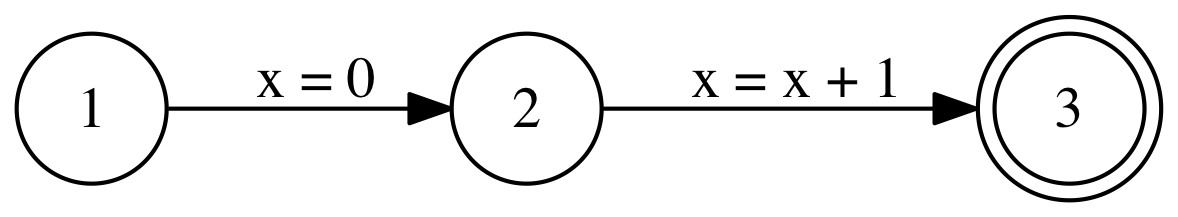
\includegraphics[width=0.7\textwidth]{sections/algorithm/images/simple-cfg}
\end{figure}

It represents the following simple JavaScript program:

\begin{minted}[linenos,xleftmargin=0.6cm]{js}
var x = 0;
x = x + 1;
\end{minted}

The abstract syntax tree in ESTree format looks like this:

\begin{minted}[linenos,baselinestretch=0.93,xleftmargin=0.75cm]{json}
{
  "type": "Program",
  "body": [
    {
      "type": "VariableDeclaration",
      "declarations": [
        {
          "type": "VariableDeclarator",
          "id": {
            "type": "Identifier",
            "name": "x"
          },
          "init": {
            "type": "Literal",
            "value": 0
          }
        }
      ],
      "kind": "var"
    },
    {
      "type": "ExpressionStatement",
      "expression": {
        "type": "AssignmentExpression",
        "operator": "=",
        "left": {
          "type": "Identifier",
          "name": "x"
        },
        "right": {
          "type": "BinaryExpression",
          "operator": "+",
          "left": {
            "type": "Identifier",
            "name": "x"
          },
          "right": {
            "type": "Literal",
            "value": 1
          }
        }
      }
    }
  ]
}
\end{minted}

\subsubsection{Parsing Statements and Expressions}

Every JavaScript program's abstract syntax tree in ESTree format has a root node of type \code{Program} with a \code{body} property that contains an array of all the main program's statements. The simple JavaScript program at the end of the previous section consists of two statements: a variable declaration and an expression statement. \code{x = x + 1} is an assignment expression and therefore not a statement on its own, but since it appears in statement position, the expression is treated as a statement of type \code{ExpressionStatement}.

The process of traversing the abstract syntax tree and deriving a control flow graph from the statements and expressions encountered can be nicely broken up into many functions, each of which knows how to parse a specific node type. One such function can call another to parse the various components of the node it knows how to parse, thereby creating a hierarchy of nested function calls. For example, the aforementioned program could be parsed by a function call hierarchy similar to the following pseudocode:

\begin{Verbatim}[xleftmargin=0.5cm]
- parseProgram()
    - parseStatements()
        - parseStatement()
            - parseVariableDeclaration()
                - parseVariableDeclarators()
                    - parseVariableDeclarator()
                        - parseInit()
                            - parseExpression()
                                - parseLiteral()
                        - parseIdentifier()
        - parseStatement()
            - parseExpressionStatement()
                - parseExpression()
                    - parseAssignmentExpression()
                        - parseRightHandSide()
                            - parseBinaryExpression()
                                - parseLeftHandSide()
                                    - parseIdentifier()
                                - parseRightHandSide()
                                    - parseLiteral()
                                - parseOperator()
                        - parseLeftHandSide()
                            - parseIdentifier()
                        - parseOperator()
\end{Verbatim}

In most cases, every expression statement adds to the control flow graph a new node with an incoming edge that is annotated with the expression. An exception to that rule, however, are expression statements that wrap expressions of type \code{SequenceExpression}.\footnote{A sequence expression as specified by ESTree \cite{estree-spec} consists of two or more expressions, separated by the comma operator, and evaluates to the value of its last expression.} Rather than adding a single node, an individual node is added for each expression in the sequence, which slightly reduces the complexity of those edge annotations in the control flow graph.

\subsubsection{Composing Structural Patterns}
\label{sec:composing-structural-patterns}

A control flow graph is created by composing various primitive patterns for statements and expressions. The following figures show a couple of examples for common control structures like conditions and loops:

\begin{figure}[h]
  \centering
  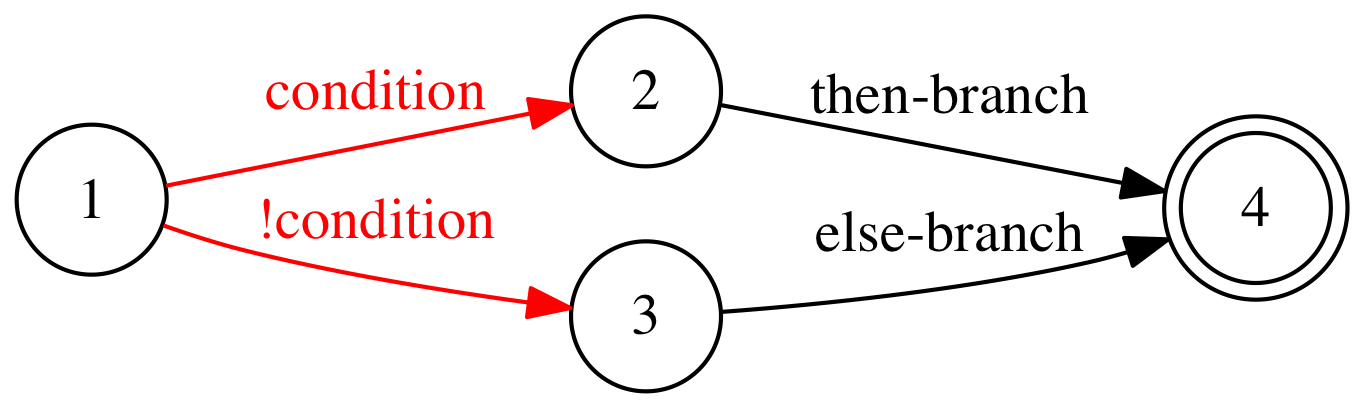
\includegraphics[width=0.7\textwidth]{sections/algorithm/images/if-else}
  \caption{An \code{if}-statement with an \code{else}-block}
  \label{fig:if-else-structural-pattern}
\end{figure}

\begin{figure}[h]
\noindent\begin{minipage}[t]{0.50\textwidth}
  \centering
  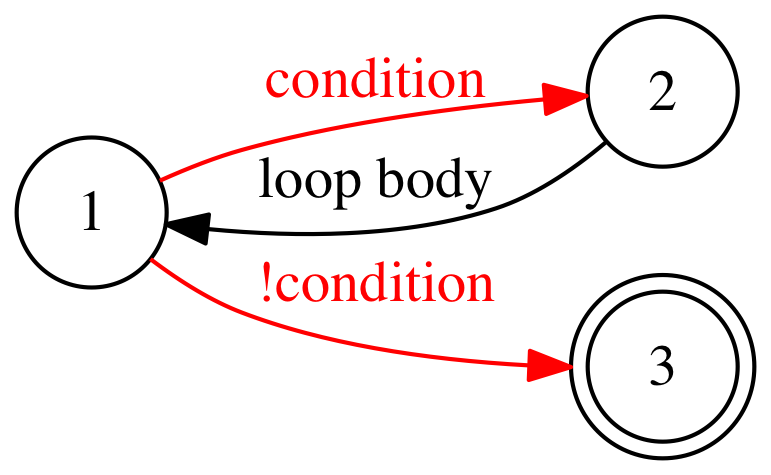
\includegraphics[width=0.8\textwidth]{sections/algorithm/images/while}
  \caption{A \code{while}-loop}
\end{minipage}
\begin{minipage}[t]{0.50\textwidth}
  \centering
  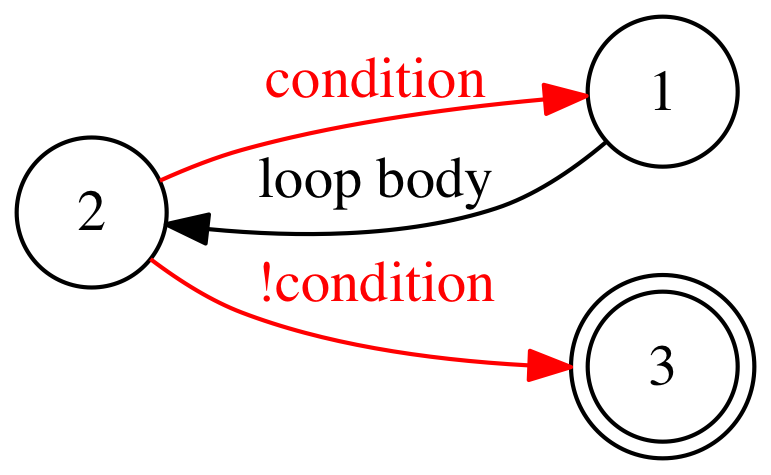
\includegraphics[width=0.8\textwidth]{sections/algorithm/images/do-while}
  \caption{A \code{do-while}-loop}
\end{minipage}
\end{figure}

\begin{figure}[h]
  \centering
  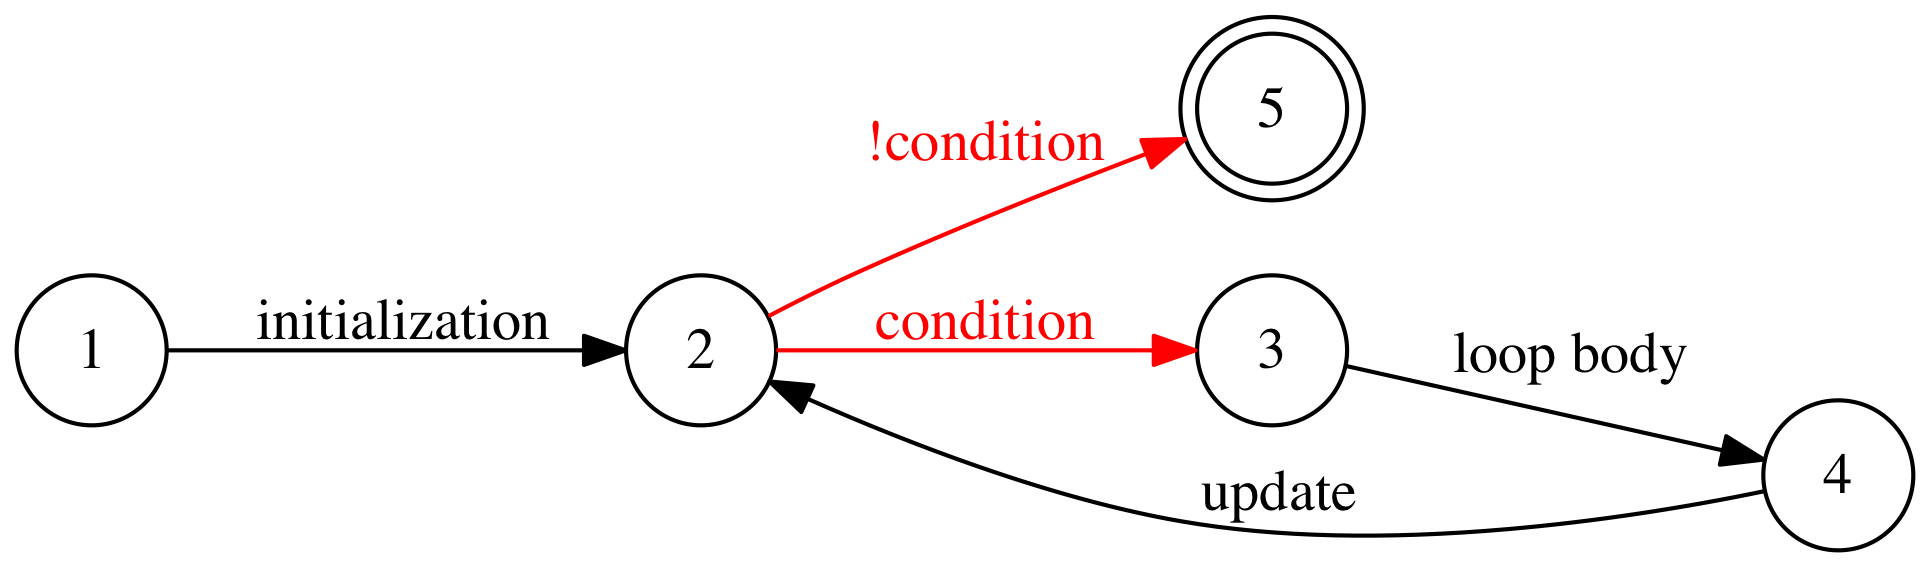
\includegraphics[width=\textwidth]{sections/algorithm/images/for}
  \caption{A \code{for}-loop}
\end{figure}

Each pattern starts with node \#1 and ends with the node that has a double border. In the above figures, those final nodes only have a double border for the purposes of clarification; they are regular nodes in the control flow graph. When two consecutive patterns are combined, the final node of the first becomes the entry node of the second. The black edges that are labeled \emph{then-branch}, \emph{else-branch}, and \emph{loop body} represent the bodies of the control structures. They can consist of arbitrarily many statements, which can contain further nested structures themselves. Similarly, \emph{initialization} and \emph{update} can hold arbitrarily complex expressions. For example, a \code{for}-loop can have a sequence expression like \code{i++, j-{}-} as its update component.

The red edges represent conditional transitions. A node that is not a final node must have either exactly one unconditional outgoing edge or exactly two conditional outgoing edges. For a pair of conditional edges, the condition is evaluated only once. Depending on whether the result is truthy or falsy\footnote{JavaScript has six values that are considered falsy: \code{undefined}, \code{null}, \code{false}, \code{0} (zero), \code{NaN} ("not a number"), and \code{""} (empty string). All other values are considered truthy.}, the corresponding conditional edge is taken.

\nameref{sec:appendix} presents a larger program and its control flow graph.

\subsubsection{Simplifying Negated Conditions}

As Figure \ref{fig:if-else-structural-pattern} in section \ref{sec:composing-structural-patterns} (``\nameref{sec:composing-structural-patterns}'') shows, an \code{if}-statement with an \code{else}-block is represented by a control flow structure that has two conditional edges. One is taken when the condition is truthy (the \emph{then-branch}), the other when it is falsy (the \emph{else-branch}). The following listing illustrates this situation:

\begin{minted}[linenos,xleftmargin=0.75cm]{js}
if (x < 0) {
    // ...
} else {
    // ...
}
\end{minted}

The then-branch is taken when \code{x < 0} returns a truthy value. It might therefore seem intuitive to assume the else-branch to be taken if and only if \code{x >= 0} is truthy. However, the precise semantics are slightly different. The else-branch is taken if and only if \code{x < 0} returns a falsy value. In general, the correct negation of \code{x < 0} is not \code{x >= 0}, but \code{!(x < 0)}. The reason for this seemingly odd behavior is that JavaScript defines some special values for which no reasonable comparison can be done using relational operators. \code{NaN} and \code{undefined} are two such values for which no sound order relation is defined.

\newpage

The following relational comparisons against \code{NaN} and \code{undefined} illustrate why the condition cannot be safely inverted (without changing the semantics of the program) by swapping the operator accordingly:

\begin{minted}[linenos,xleftmargin=0.75cm]{js}
NaN <  0   // false
NaN >  0   // false
NaN <= 0   // false
NaN >= 0   // false

undefined <  0   // false
undefined >  0   // false
undefined <= 0   // false
undefined >= 0   // false
\end{minted}

This observation prevents some simplification of conditional edges in a control flow graph. To stay true to the program semantics, the conditional annotation of the edge transitioning into the else-branch must be \code{!(x < 0)} (rather than the simpler \code{x >= 0}) to account for those special values.

However, some simplification of expressions is possible. Both the equality comparison operators (\code{==} and \code{!=}) and the identity comparison operators (\code{===} and \code{!==}) can safely be negated by flipping the first character from an equal sign to an exclamation mark, and vice-versa. Also, two consecutive applications of the unary negation operator (\code{!}) cancel each other out and do not affect the truthiness of a value. Therefore, the following simplifications are safe and do not affect the semantics of the program:

\begin{minted}[linenos,xleftmargin=0.75cm]{js}
// Simplifying a negated identity comparison
!(x === 0)
x !== 0

// Simplifying a negated inequality comparison
!(x != 0)
x == 0

// Canceling out a double negative
!!(x)
x
\end{minted}

Nota bene: The above simplifications are only semantically correct w.r.t. the evaluation of the expression to a truthy or falsy value, as is the case when evaluating the condition of an \code{if}-statement. The simplifications do not necessarily result in an identical value or even a value of the same type. For instance, the unary negation operator coerces its operand into a boolean value. Therefore, \code{!!0}, which evaluates to the boolean value \code{false} (because \code{!0} evaluates to \code{true}), is not identical to \code{0}, which is a numeric value. Both are falsy values, though, and thus direct control flow correctly.

